% Please use the skeleton file you have received in the
% invitation-to-submit email, where your data are already
% filled in. Otherwise please make sure you insert your
% data according to the instructions in PoSauthmanual.pdf
\documentclass[a4paper]{jpconf}
\usepackage{graphicx}
\usepackage{epstopdf} 
\begin{document}

\title{Liquid Argon optical properties to be used in Geant4 and Opticks Simulations}

\author{ Hans~Wenzel$^1$}

\address{ $^1$~Fermilab PO Box 500, Batavia, IL 60510,
USA}

\ead{wenzel@fnal.gov}

\begin{abstract}
  In Geant4 and Opticks optical properties like e.g. the materials refractive
  index are inputs that have to be provided. In this paper we collect the
  optical properties relevant for liquid Argon TPC's.   
\end{abstract}

\section{Introduction}
  In Geant4 and Opticks optical properties like e.g. the materials refractive
  index are inputs that have to be provided. In this article we briefly describe the physical processes relevant to the
  production, transport and detection of optical photons in liquid Argon. We collect the
  values and parameterizations of optical properties relevant for liquid Argon TPC's. We provide scripts that plot this quantities and that convert this values
  into a gdml description that can be directly used in the Geant4 Detector description.
  All values are summarized in the file material.xml which can be found in the github repository \cite{ref:scripts}.
  Usually quantities are given as a funcyion of photon wavelength but Geant4 requires the photon energy.
  
\begin{equation}
  E_{\gamma} = \frac{h * c}{\lambda_{\gamma} * 1.e-9}
  \label{equ:equation1}
\end{equation}
  const double c = 299792458.;         // speed of light in m/sec
  const double h = 4.13566743E-15;     // Planck constant in eVsec
  
  \section{Light production}  
  \subsection{Scintillation Properties of liquid Argon}
  Light yield ~ few 10,000’s of photons per MeV (depends on E field, particle type and purity)
(SCINTILLATIONYIELD: 50000/MeV when no electric field present)
  \begin{table}[h!]
  \begin{center}
    \label{tab:table1}
    \begin{tabular}{|l|c|} % <-- Alignments: 1st column left, 2nd middle and 3rd right, with vertical lines in between
      \hline
      \textbf{Property/Geant4 property} &       \textbf{value}\\
      \hline
      yield/SCINTILLATIONYIELD & 50000 photons/MeV (no electric field)\\
      Wavelength of emission &  128nm (FWHM=10nm)\\
      fast component/SCINTILLATIONTIMECONSTANT1& 6 ns\\  
      fast fraction/SCINTILLATIONYIELD1& 0.75 \\
      slow component/SCINTILLATIONTIMECONSTANT2& 1500 ns \\
      slow fraction/SCINTILLATIONYIELD2& 0.25\\
      RESOLUTIONSCALE& 1\\
      \hline
    \end{tabular}
  \end{center}
  \caption{Scintillation Properties of liquid Argon.}
  \end{table}

\subsection{Cerenkov spectrum and Yield}
\begin{figure}
\centering
\begin{minipage}{.5\textwidth}
  \centering
  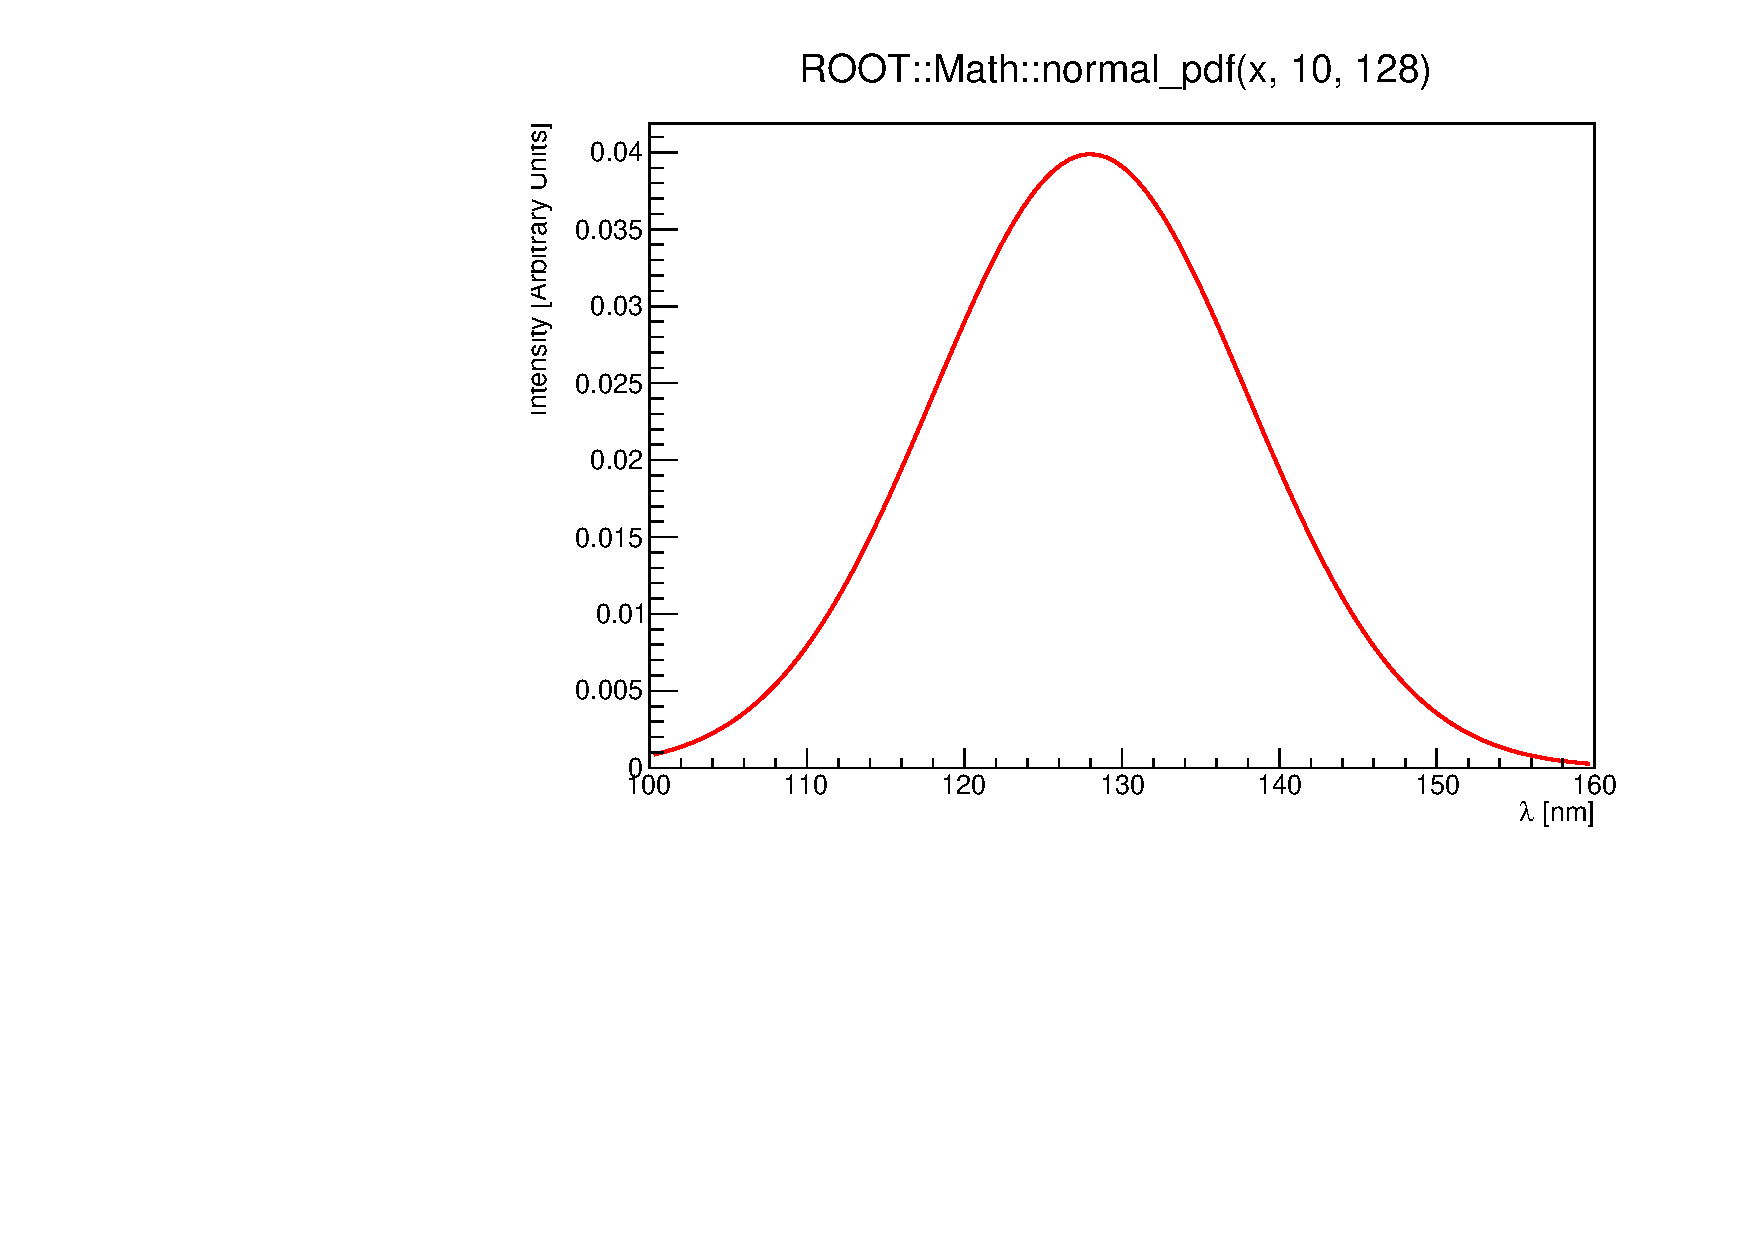
\includegraphics[width=.7\linewidth]{spectrum.pdf}
%  \captionof{figure}{A figure}
%  \label{fig:spectrum}
\end{minipage}%
\begin{minipage}{.5\textwidth}
  \centering
  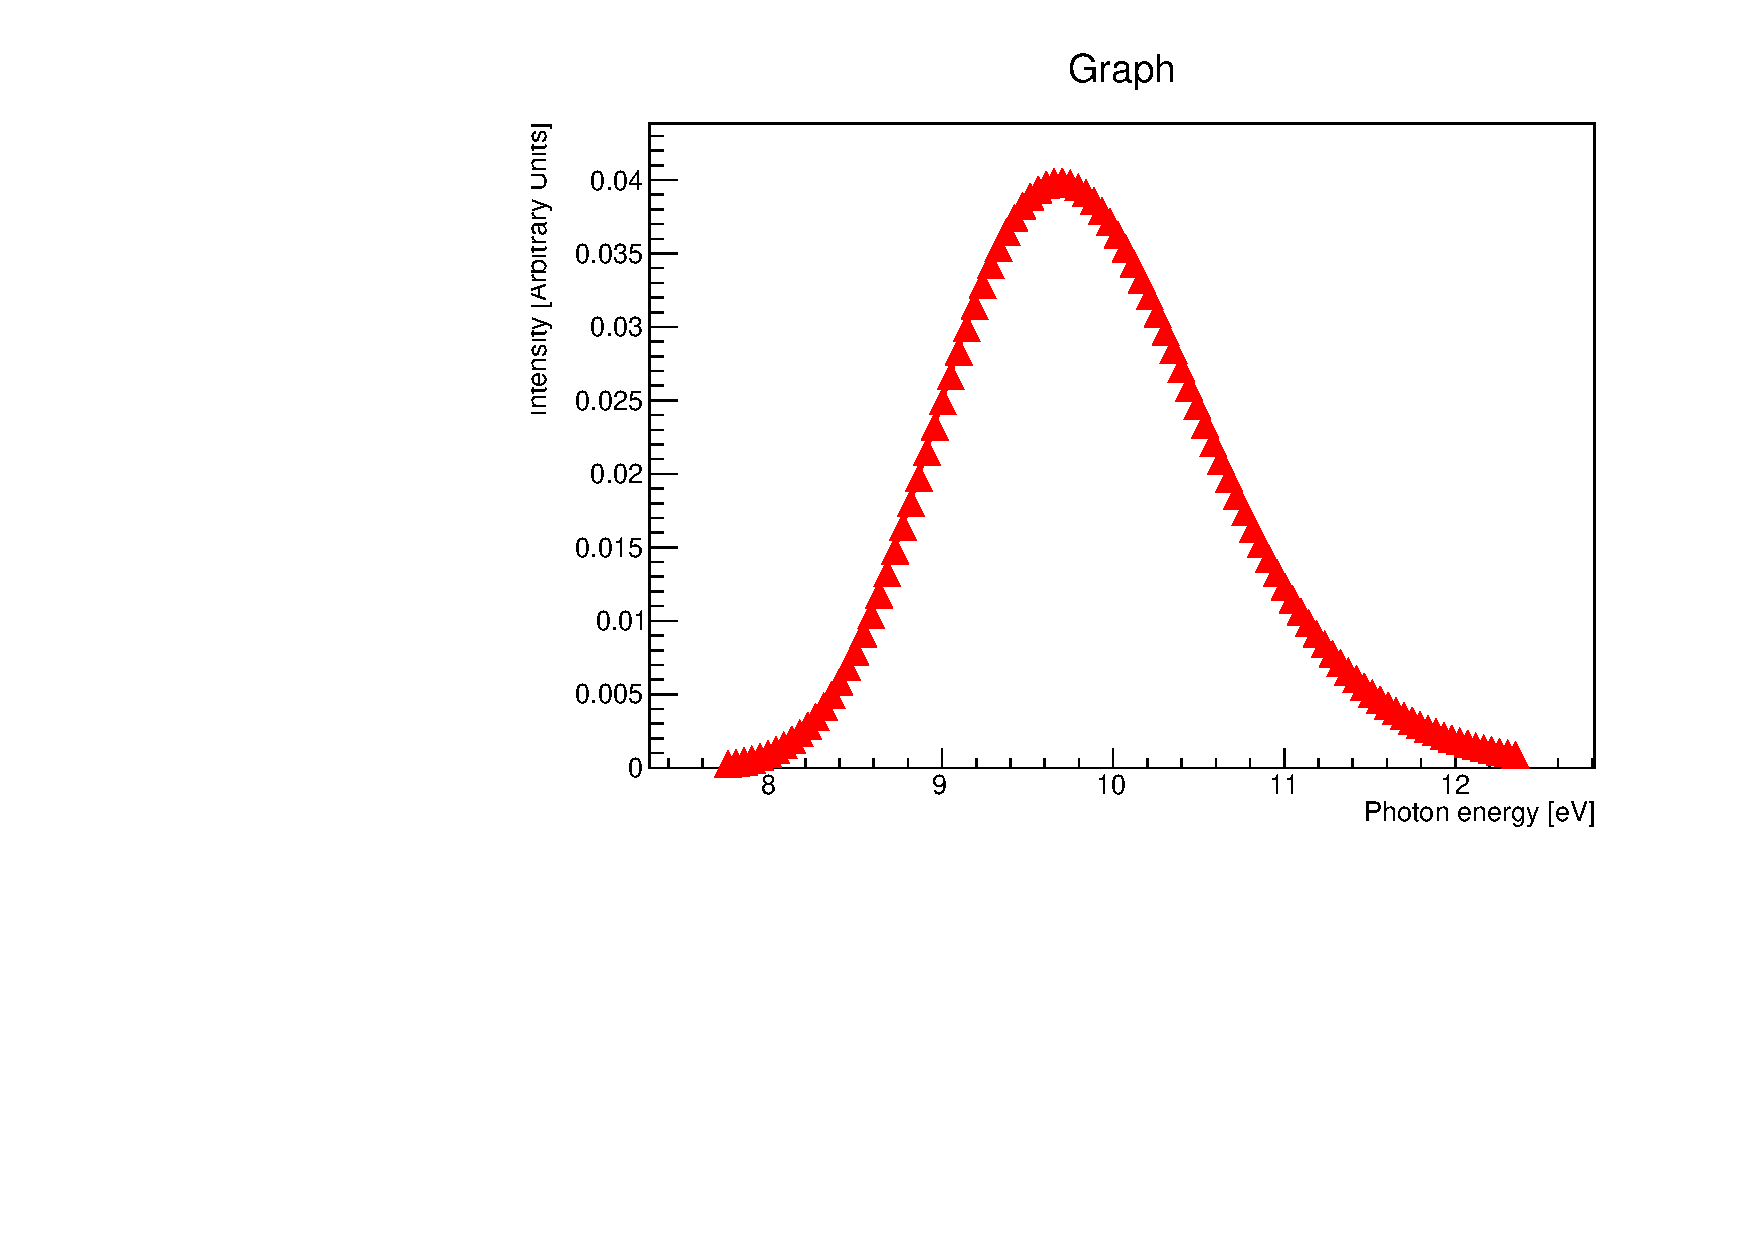
\includegraphics[width=.7\linewidth]{spectrumE.pdf}
%  \captionof{figure}{Another figure}
%  \label{fig:spectrumE}
\end{minipage}
\caption{\label{fig:spectrum}Scintillation emmission spectrum.}
\end{figure}

\section{Light propagation}
\subsection{Refraction Index of liquid Argon}
\begin{equation}
  v_g (\lambda)= \frac{c}{n-\lambda \frac{\partial{n}}{\partial{\lambda}}}
      \label{equ:vgroup}
% \caption{relation between refraction index and group velocity.}       
\end{equation}
Refraction Index: $n = 1.358 \pm 0.003 at 128 nm$ (M. Babicz et al 2020 JINST 15 P09009)
                            ( compared to $n= 1.45 \pm 0.07$ (ArXiv:1502.04213))
Group velocity: $1/ vg = 7.46 \pm 0.08 ns/m at 128 nm$
\begin{equation}
n^2 = a_0 + \frac{a_{UV} \lambda^2}{\lambda^2 -\lambda^2_{UV}}+\frac{a_{IR}\lambda^2}{\lambda^2 - \lambda^2_{IR}}.
 \label{equ:sellmeier}
\end{equation}

% \caption{relation between refraction index and group velocity.} 
\begin{figure}[ht]
\begin{center}
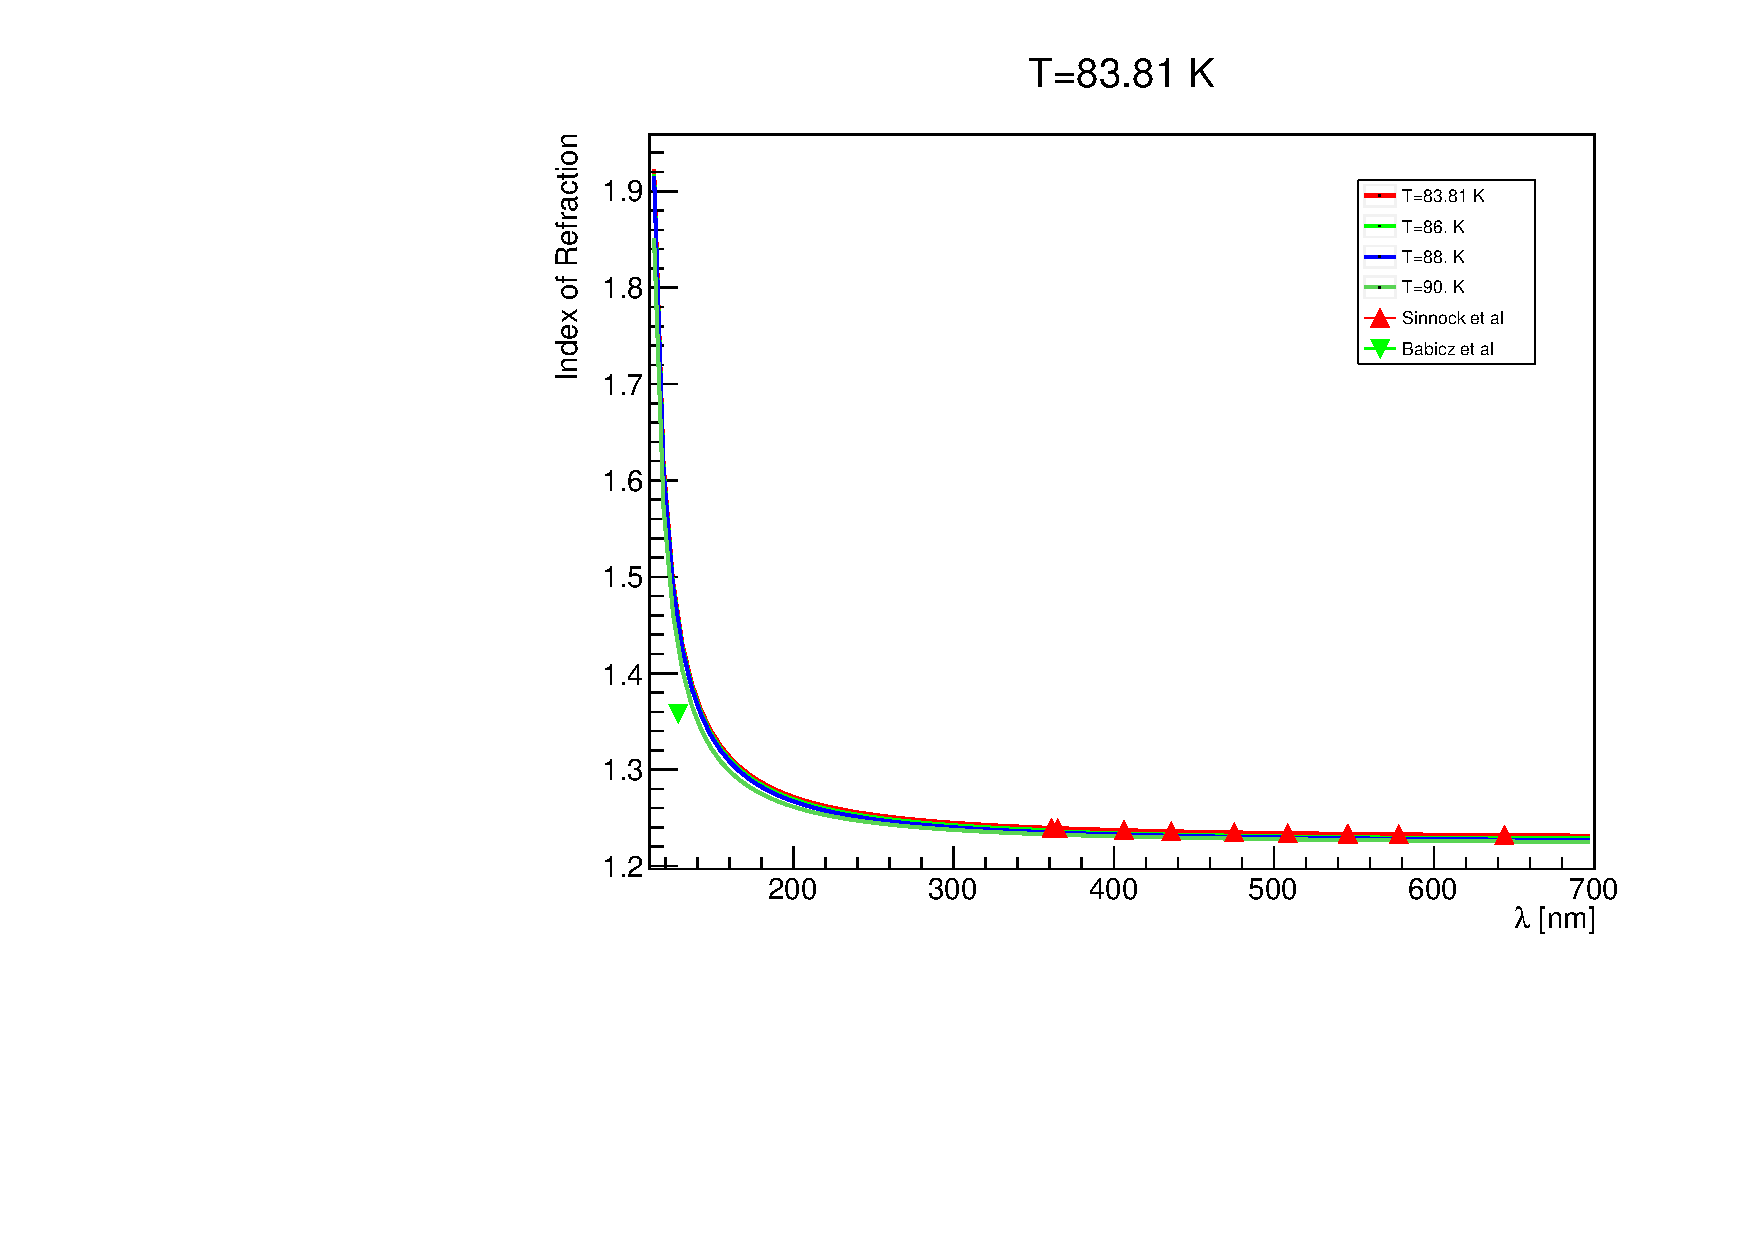
\includegraphics[width=35.5pc]{sellmeier.pdf}
\end{center}
\caption{\label{fig:sellmeier.pdf}refraction index}
\end{figure}

\subsection{Absorption length}
Argon is highly transparent to its own scintillation light. (ABSLENGTH)
  $> 1.1 m$  (ArXiv:1511.07725) 
  \subsection{Rayleigh Scattering length}
  Rayleigh scattering length (RAYLEIGH): 90 cm (M. Babicz et al 2020 JINST 15 P09009)
  $55\pm  5 cm$ (ArXiv:1502.04213)

  \begin{figure}[ht]
    \begin{center}
      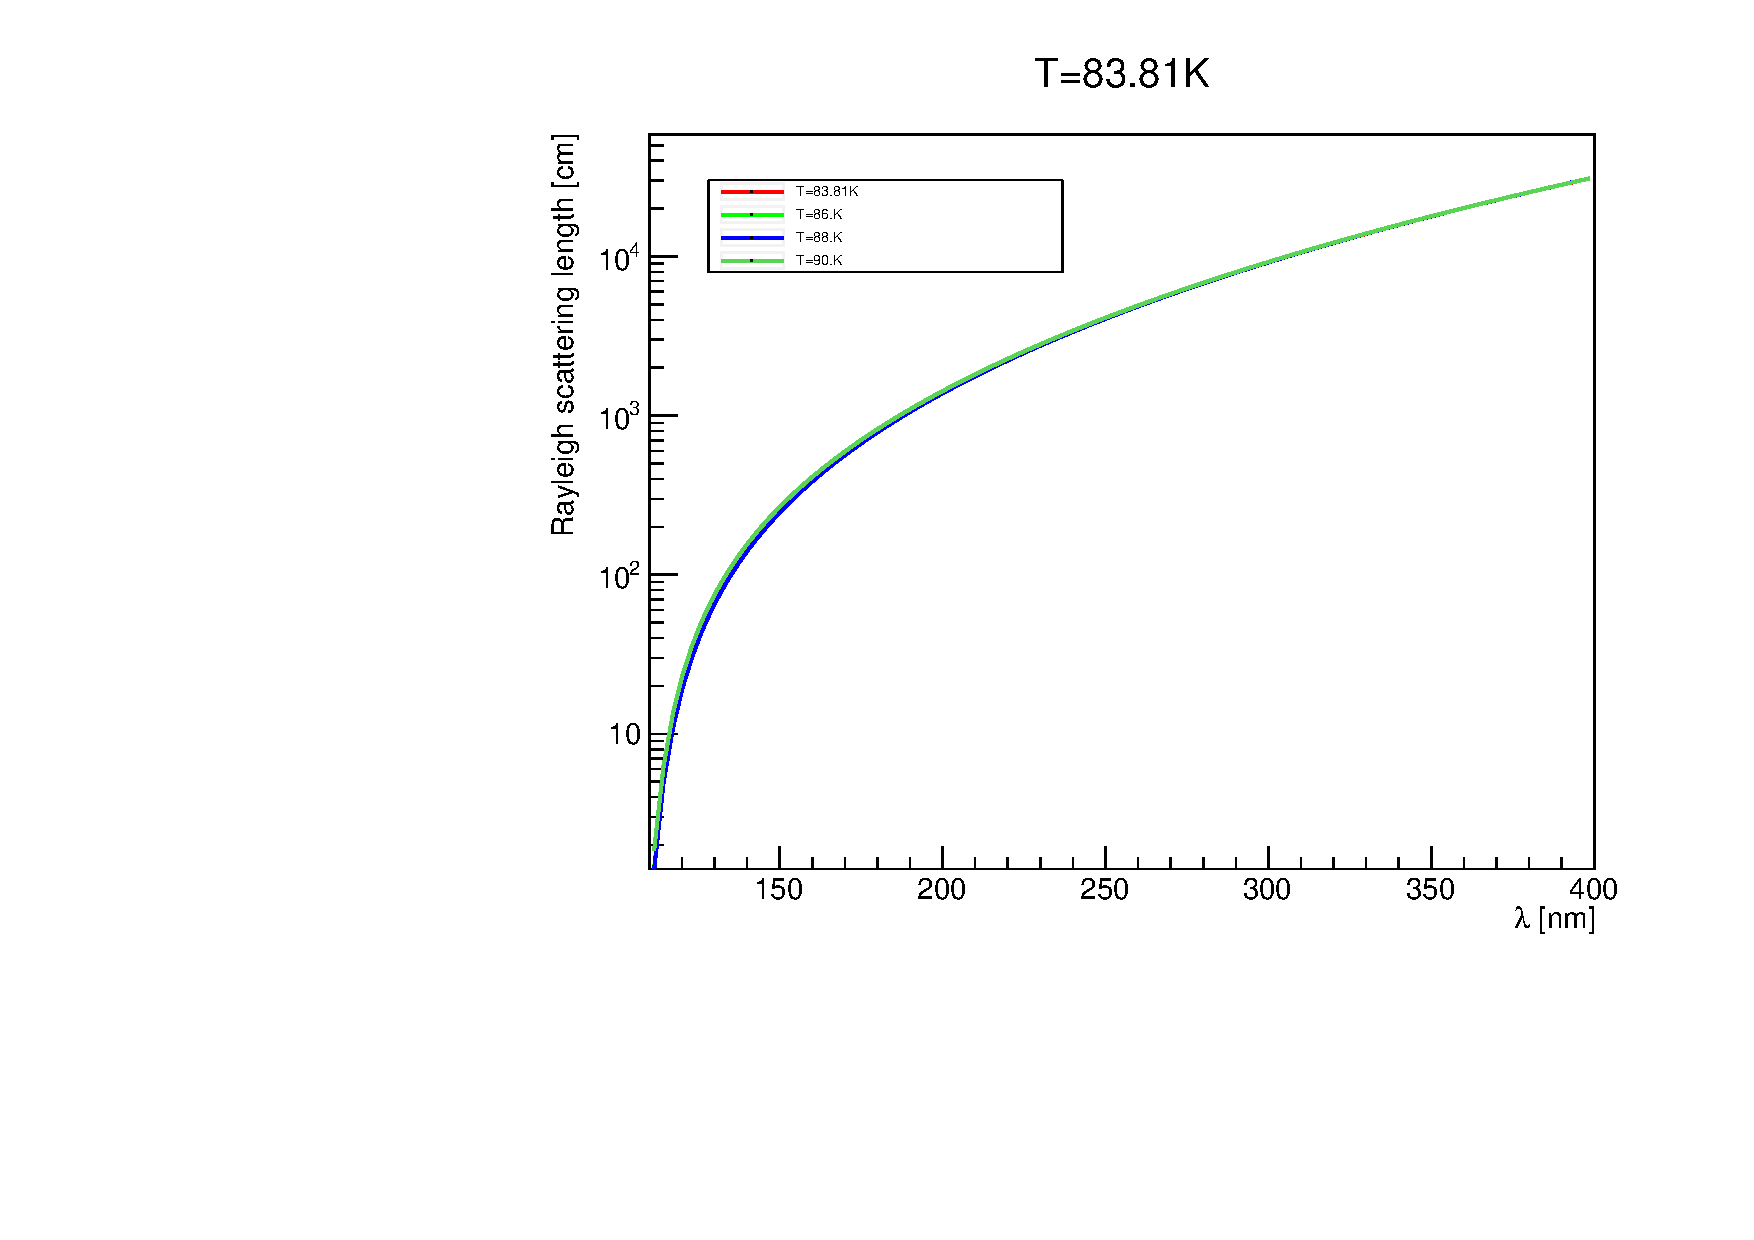
\includegraphics[width=35.5pc]{rayleigh.pdf}
    \end{center}
    \caption{\label{fig:rayleigh}rayleigh scattering length.}
  \end{figure}
  
  \section{Photon Detection}
  
\subsection{Quantum efficiency and absorption length of the tetraphenyl butadiene wave length shifter}
\cite{ref:wls}
\begin{figure}[ht]
\begin{center}
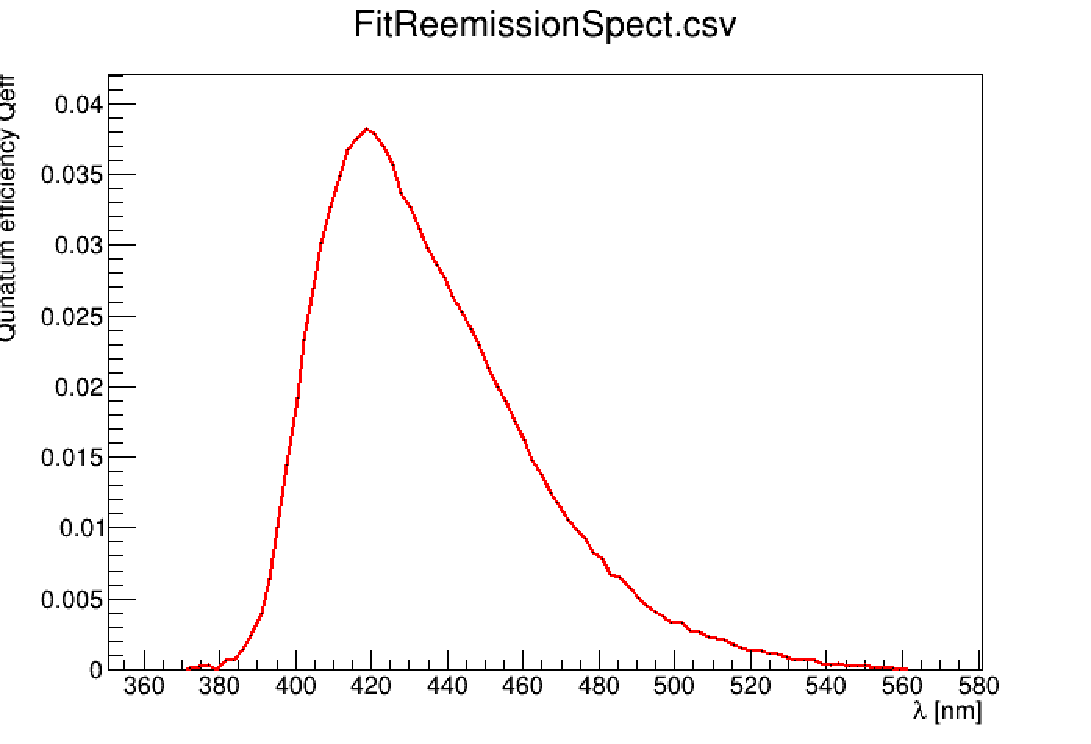
\includegraphics[width=35.5pc]{wls.pdf}
\end{center}
\caption{\label{fig:wls}wave length spectrum extracted form \cite{ref:wls}.}
\end{figure}

\section{Quantum efficiency and absorption length of the tetraphenyl butadiene wave length shifter}

\section{Conclusions and Outlook}

 \section*{References}

 \begin{thebibliography}{99}
 \bibitem{ref:LArProperties}
   \verb|https://github.com/hanswenzel/LArProperties|.
 \bibitem{ref:CaTS}
   \verb|https://github.com/hanswenzel/CaTS|.
\bibitem{ref:Geant4-4}
 Allison J et al. 2016, {\it Nuclear Instruments and Methods in Physics
                Research A} {\bf 835} (186--225).
\bibitem{ref:Geant4}
 \verb|http://geant.cern.ch/|.
\bibitem{ref:inspire} High-Energy Physics Literature Database,
  \verb"http://inspirehep.net"/.
\bibitem{ref:scripts}  
  \verb|https://github.com/hanswenzel/CaTS/tree/master/scripts/LAr.C|.\\
  \verb|https://github.com/hanswenzel/CaTS/tree/master/scripts/wls.C|.

\bibitem{ref:wls} Christopher Benson, Gabriel D. Orebi Gann, Victor Gehman,\\
  {\it Measurements of the intrinsic quantum efficiency and absorption
      length of tetraphenyl butadiene thin films in the vacuum
      ultraviolet regime.}\\
Eur. Phys. J. C (2018) 78:329
\bibitem{grace}Emily Grace, Alistair Butcher, Jocelyn Monroe, James A. Nikkel,\\
  \it{Index of refraction, Rayleigh scattering length, and Sellmeier coefficients in solid and liquid argon and xenon.}\\
  \verb|ArXiv:1502.04213|
\bibitem{gv} 
  \it{A measurement of the group velocity of scintillation light in liquid argon}
  M. Babicz et al 2020 JINST 15 P09009
\bibitem{ben}
  Ben Jones, \it{Introduction to Scintillation Light in Liquid Argon}
  \verb''http://microboone-exp.fnal.gov''/
  \bibitem{morikawa}E. Morikawa, R. Reininger, P. Gürtler, V. Saile, and P. Laporte,\\
\it{Argon, krypton, and xenon excimer luminescence: From the dilute gas to the
condensed phase.}\\
J. Chem. Phys. 91, 1469 (1989);
  \verb|https://doi.org/10.1063/1.457108|


  
\end{thebibliography}

\end{document}
